%!TEX program = xelatex
\documentclass[a4paper,12pt]{report}
\usepackage{ctex}
%\usepackage{xeCJK}
\usepackage{times}
\usepackage{graphicx,float}
\usepackage{setspace}
\usepackage{fancyhdr}
% \usepackage{graphicx}
\usepackage{wrapfig}
\usepackage{array}
\usepackage{fontspec,xunicode,xltxtra}
\usepackage{titlesec}
\usepackage{titletoc}
\usepackage[titletoc]{appendix}
\usepackage[top=30mm,bottom=30mm,left=20mm,right=20mm]{geometry}
\usepackage{cite}
\usepackage{listings}
\usepackage{xcolor}
\usepackage[framed,numbered,autolinebreaks,useliterate]{mcode} % 插入代码
\XeTeXlinebreaklocale "zh"
\XeTeXlinebreakskip = 0pt plus 1pt minus 0.1pt

%---------------------------------------------------------------------
%	页眉页脚设置
%---------------------------------------------------------------------
\fancypagestyle{plain}{
	\pagestyle{fancy}      %改变章节首页页眉
}

\pagestyle{fancy}
\lhead{\kaishu~``高级语言编程实训''实验报告~}
\rhead{\kaishu~~Anonymous~Anonymous~Anonymous~}
\cfoot{\thepage}

%---------------------------------------------------------------------
%	章节标题设置
%---------------------------------------------------------------------
\titleformat{\chapter}{\centering\zihao{-1}\heiti}{实验\chinese{chapter}}{1em}{}
\titlespacing{\chapter}{0pt}{*0}{*6}

%---------------------------------------------------------------------
%	摘要标题设置
%---------------------------------------------------------------------
\renewcommand{\abstractname}{\zihao{-3} 摘\quad 要}

%---------------------------------------------------------------------
%	参考文献设置
%---------------------------------------------------------------------
\renewcommand{\bibname}{\zihao{2}{\hspace{\fill}参\hspace{0.5em}考\hspace{0.5em}文\hspace{0.5em}献\hspace{\fill}}}

%---------------------------------------------------------------------
%	引用文献设置为上标
%---------------------------------------------------------------------
\makeatletter
\def\@cite#1#2{\textsuperscript{[{#1\if@tempswa , #2\fi}]}}
\makeatother

%---------------------------------------------------------------------
%	目录页设置
%---------------------------------------------------------------------
\titlecontents{chapter}[0em]{\songti\zihao{-4}}{\thecontentslabel\ }{}
{\hspace{.5em}\titlerule*[4pt]{$\cdot$}\contentspage}
\titlecontents{section}[2em]{\vspace{0.1\baselineskip}\songti\zihao{-4}}{\thecontentslabel\ }{}
{\hspace{.5em}\titlerule*[4pt]{$\cdot$}\contentspage}
\titlecontents{subsection}[4em]{\vspace{0.1\baselineskip}\songti\zihao{-4}}{\thecontentslabel\ }{}
{\hspace{.5em}\titlerule*[4pt]{$\cdot$}\contentspage}

\renewcommand\thesection{\arabic{section}}
\renewcommand\thesubsection{\arabic{section}.\arabic{subsection}}

\begin{document}
%---------------------------------------------------------------------
%	封面设置
%---------------------------------------------------------------------
\begin{titlepage}
	\begin{center}
		
    
\includegraphics[width=1.0\textwidth]{figure//nankai.jpg}\\
    % \vspace{10mm}
    % \textbf{\zihao{2}\kaishu{软件学院}}\\[0.8cm]
    \vspace{50mm}
    \textbf{\zihao{1}\heiti{ 《高级语言编程实训》实验报告}}\\[3cm]

	\vspace{\fill}
	
\setlength{\extrarowheight}{3mm}
{\songti\zihao{3}	
\begin{tabular}{rl}
	
	{\makebox[4\ccwd][s]{学\qquad 院:}}& ~\kaishu 软件学院\\
	
	{\makebox[4\ccwd][s]{姓\qquad 名:}}& ~\kaishu Anonymous~Anonymous~Anonymous \\

    {\makebox[4\ccwd][s]{学\qquad 号:}}& ~\kaishu Anonymous~Anonymous~Anonymous \\

	{\makebox[4\ccwd][s]{指导老师:}} & ~\kaishu Anonymous~Anonymous\\

\end{tabular}
 }\\[2cm]
\vspace{\fill}
\zihao{4}
2020\textasciitilde 2021夏季学期\\
使用\LaTeX 撰写于\today
	\end{center}	
\end{titlepage}


%---------------------------------------------------------------------
%  目录页
%---------------------------------------------------------------------
\tableofcontents % 生成目录

%---------------------------------------------------------------------
%  实验一
%---------------------------------------------------------------------
\chapter*{星露谷物语的实现}
\setcounter{page}{1}
\begin{spacing}{1.5}
\songti\zihao{-4}

\section{分工情况}
 \begin{itemize}
 	\item 薛湛童:游戏代码编写
 	\item 王佳慧:游戏地图制作,PPT制作,课堂展示
 	\item 吴贤伟:实验报告书写
 \end{itemize}
\section{软件介绍}
该软件是我们对单机游戏星露谷物语的复刻版本,这是一款开放式乡村模拟经营类游戏,游戏中玩家扮演继承了爷爷农场的“Stardew valley”主角开阔和经营整座小牧场;游戏采用了像素的风格,
在如今大作如云的时代可能并不能收所有玩家喜爱,但是其超高开放度的自由游玩和清新自然的游戏风格依旧吸引着许多怀旧玩家,本软件在很大程度上还原了游戏本身,也可以带来很棒的游戏体验。
\subsubsection{代码GitHub地址}
软件的GitHub地址为https://github.com/listerily/qt-practice-assignment
\section{想法来源}
该软件制作想法来源于小组成员对星露谷物语的游玩体验,过程中,我们被其清新自然的游戏风格深深吸引,游戏本身带给我们的乐趣是我们决定一起开发这款游戏的最大推动力,我们的目标就是尽可能还原
这种极佳的游戏体验。

\section{心得体会}
通过编写该软件我们深深体会到游戏开发的不易,日常生活中,我们可能更多关注自己的游玩体验,对于软件的开发并不关心,更不知道背后工作人员所付出的努力,在这个过程中,我们体验了程序员开发游戏
的部分过程;与此同时,我们也感受到团队合作的重要性,作为团队的一员,我们每个人必需为推动整个项目付出自己的努力,也需要明确分工,彼此加强沟通与交流,这样整个团队的工作效率才会提高,游戏开发的
质量才会有保障;在这个过程中,我们也在一定程度上锻炼了自己的编程能力,是对于理论课知识很好的实践,我们每个人也都很享受这个过程。
\end{spacing}

\section{软件截图}
\zihao{-4}\songti
\begin{spacing}{1.5}
软件截图如图~\ref{pic1}所示。

\begin{figure}[H]
  \centering
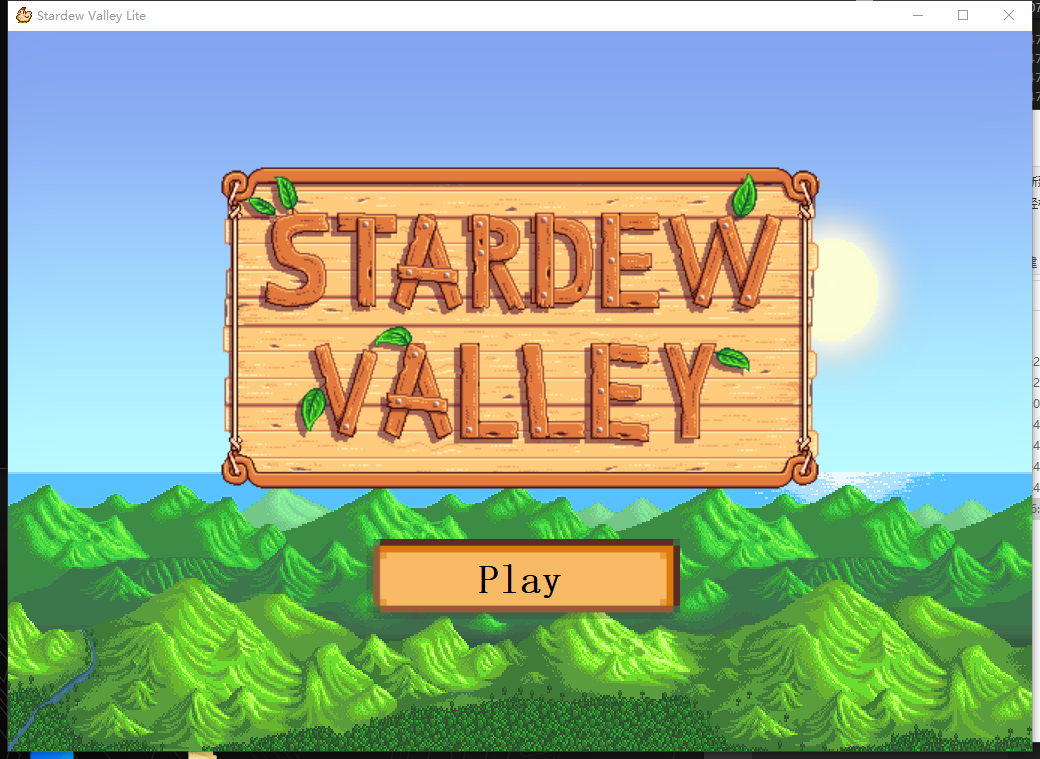
\includegraphics[width=3.3in]{3.png}\caption{开始界面}\label{pic1}
\end{figure}

\begin{figure}[H]
  \centering
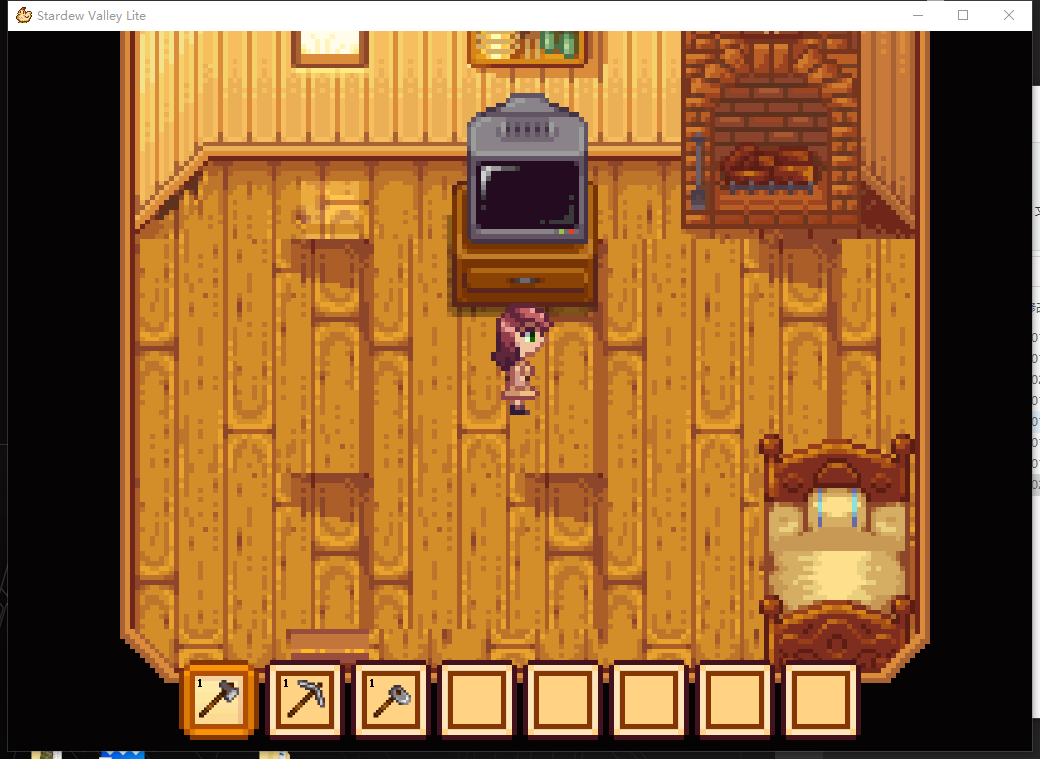
\includegraphics[width=3.3in]{4.png}\caption{家}\label{pic2}
\end{figure}

\begin{figure}[H]
  \centering
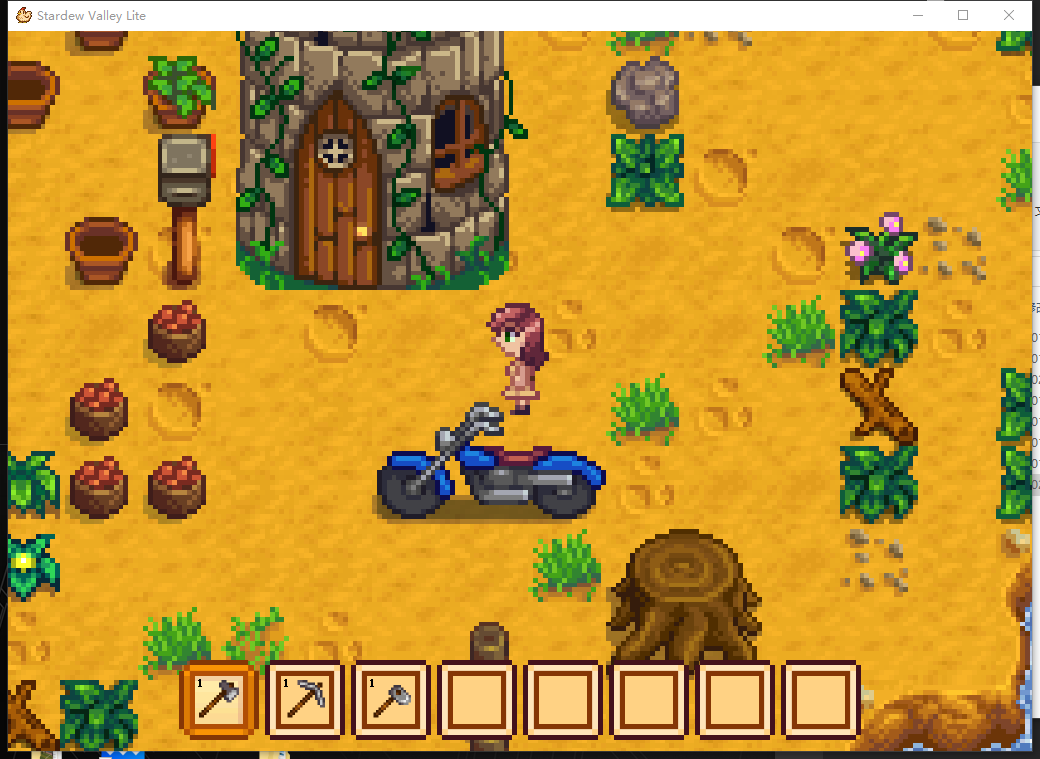
\includegraphics[width=3.3in]{2.png}\caption{外部世界}\label{pic2}
\end{figure}

\begin{figure}[H]
  \centering
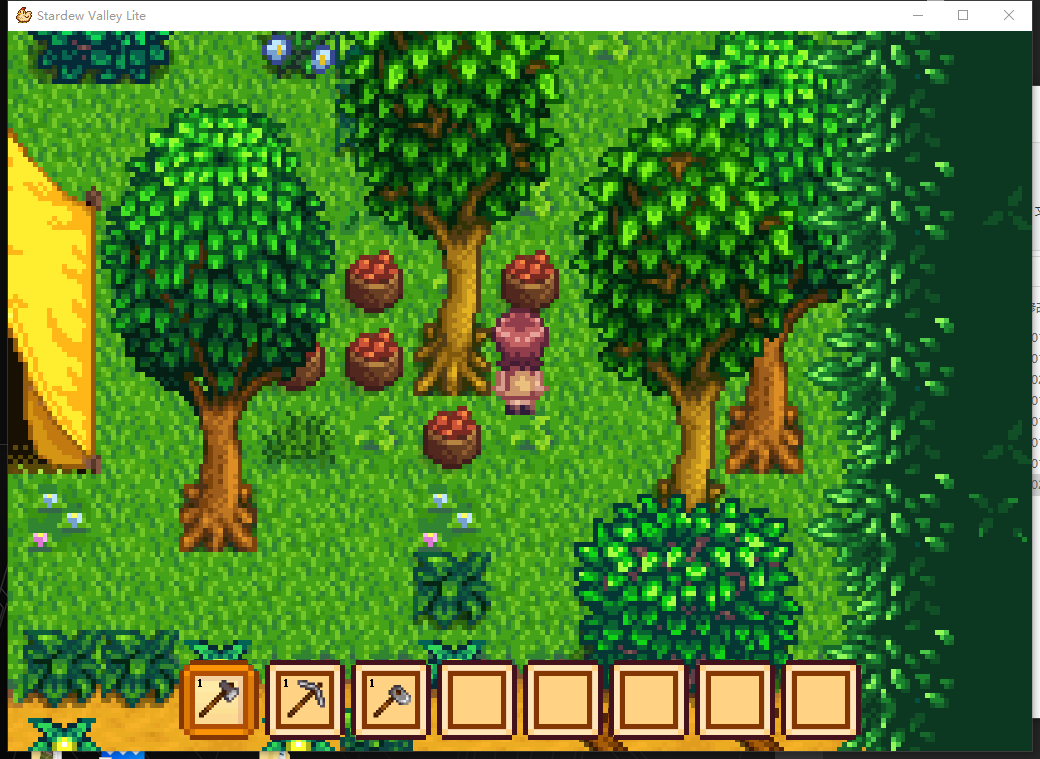
\includegraphics[width=3.3in]{5.png}\caption{森林}\label{pic2}
\end{figure}

\begin{figure}[H]
  \centering
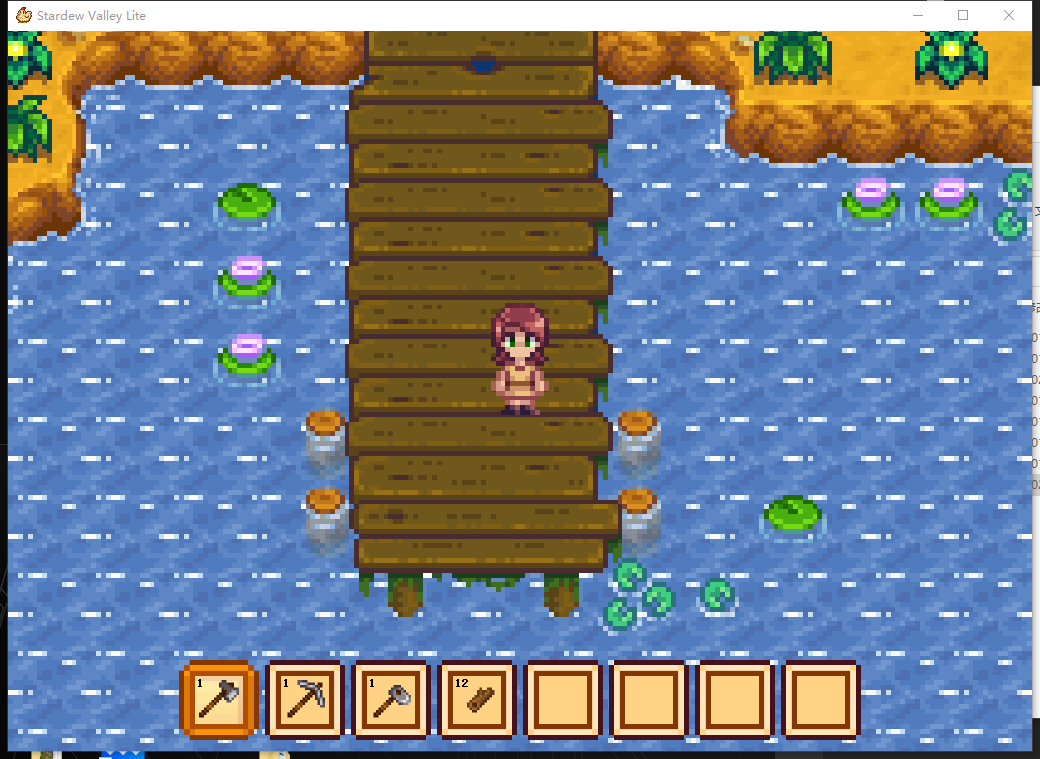
\includegraphics[width=3.3in]{1.png}\caption{小桥}\label{pic2}
\end{figure}
\end{spacing}

\lstset{
    %backgroundcolor=\color{red!50!green!50!blue!50},%代码块背景色为浅灰色
    rulesepcolor= \color{gray}, %代码块边框颜色
    breaklines=true,  %代码过长则换行
    numbers=left, %行号在左侧显示
    numberstyle= \small,%行号字体
    %keywordstyle= \color{red},%关键字颜色
    commentstyle=\color{gray}, %注释颜色
    frame=shadowbox%用方框框住代码块
    }


\section{核心代码}
\zihao{-4}\songti
\begin{spacing}{1.5}
核心代码如下:\\
\subsection{\textbf{*src/ui}}
有关用户交互和图形显示,主要窗口是GamePlayWindow,该窗口处理系统层面的用户输入事件并把它们传给游戏后端(GameClient),核心代码如下:\\
\begin{lstlisting}[language={C++}]
GamePlayWindow::GamePlayWindow(GameClient &client, QWidget *parent) :
        gameClient(client),
        QWidget(parent),
        currentWorld(*client.getCurrentWorld()),
        inputHandler(client.getInputHandler()),
        ui(new Ui::GamePlayWindow)
{
    ui->setupUi(this);
    setWindowTitle("Stardew Valley Lite");

    painter = new WorldPainter;
    currentSlotID = 0;

    buttons = {ui->button_0, ui->button_1, ui->button_2, ui->button_3, ui->button_4, ui->button_5, ui->button_6,
               ui->button_7};
    for (int i = 0; i < 8; ++i)
    {
        connect(buttons[i], &QPushButton::clicked, this, [=]() { this->slotButtonClicked(i); });
        buttons[i]->setFocusPolicy(Qt::FocusPolicy::NoFocus);
        labels[i] = new QLabel("", buttons[i]);
        labels[i]->setGeometry(18, 8, labels[i]->width(), labels[i]->height());
        labels[i]->setStyleSheet("QLabel{color:black;font-weight:bold;}");
        labels[i]->show();
    }

    selectSlot(0);

    mediaPlaylist = new QMediaPlaylist;
    mediaPlaylist->addMedia(QMediaContent
    (QUrl("qrc:/svl/audio/audio/0000005b.mp3")));
    mediaPlaylist->setPlaybackMode(QMediaPlaylist::CurrentItemInLoop);
    mediaPlayer = new QMediaPlayer(this);
    mediaPlayer->setPlaylist(mediaPlaylist);
    mediaPlayer->play();
}

void GamePlayWindow::paintEvent(QPaintEvent *event)
{
    painter->paint(gameClient, *gameClient.getCurrentWorld(), *this, width(), height());
    QWidget::paintEvent(event);
}

void GamePlayWindow::keyPressEvent(QKeyEvent *event)
{
    QWidget::keyPressEvent(event);

    inputHandler.keyPressEvent(event->key());
}

void GamePlayWindow::keyReleaseEvent(QKeyEvent *event)
{
    QWidget::keyReleaseEvent(event);

    inputHandler.keyReleaseEvent(event->key());
}

void GamePlayWindow::wheelEvent(QWheelEvent *event)
{
    QWidget::wheelEvent(event);
    painter->zoom(-event->angleDelta().y() / 60);
}

void GamePlayWindow::mousePressEvent(QMouseEvent *event)
{
    QWidget::mousePressEvent(event);
    auto &playerController = currentWorld.getPlayerController();
    if (event->button() == Qt::LeftButton)
    {
        double x = event->x();
        double y = event->y();
        double width = this->width();
        double height = this->height() + 15.0;
        double k = (double) height / width;
        if (y < k * x && y < height - k * x)
            playerController.turn(Player::Facing::UP);
        else if (y < k * x && y > height - k * x)
            playerController.turn(Player::Facing::RIGHT);
        else if (y > k * x && y > height - k * x)
            playerController.turn(Player::Facing::DOWN);
        else if (y > k * x && y < height - k * x)
            playerController.turn(Player::Facing::LEFT);

        currentWorld.getPlayerController().interact(false);
    } else if (event->button() == Qt::RightButton)
    {
        currentWorld.getPlayerController().interact(true);
    }
}
\end{lstlisting}
\subsection{\textbf{*src/ui/painter}}
\begin{itemize}
    \item 把世界上的所用东西绘画到窗口上;
    \item 渲染世界地面、玩家背后动作、玩家、玩家身前动作、世界天空;
    \item 同时动态处理displayBlocksNum实现画面缩放,动态处理width、height实现自适应窗口大小。
\end{itemize}
核心代码如下:
\begin{lstlisting}[language={C++}]
void WorldPainter::paint(const GameClient &client, const GameWorld &world, QWidget &widget, int width, int height)
{
    ++paintFrameCount;

    const auto &player = world.getPlayer();
    const auto pixelsCount = width * height;
    const auto displayBlockArea = (double) pixelsCount / displayBlocksNum;
    const auto displayBlockWidth = static_cast<int>(sqrt(displayBlockArea));
    const auto playerPositionX = player.getPosition().first;
    const auto playerPositionY = player.getPosition().second;
    const auto viewPortCenterX = width / 2.0 - (playerPositionX - floor(playerPositionX)) * displayBlockWidth;
    const auto viewPortCenterY = height / 2.0 - (playerPositionY - floor(playerPositionY)) * displayBlockWidth;
    const auto viewPortCenterTargetWorldPointX = (int) floor(playerPositionX);
    const auto viewPortCenterTargetWorldPointY = (int) floor(playerPositionY);
    const auto halfDisplayCountInWidth = (int) ceil(width / 2.0 / displayBlockWidth);
    const auto halfDisplayCountInHeight = (int) ceil(height / 2.0 / displayBlockWidth);
    const auto viewPortStartPointX = viewPortCenterX - displayBlockWidth * halfDisplayCountInWidth;
    const auto viewPortStartPointY = viewPortCenterY - displayBlockWidth * halfDisplayCountInHeight;
    const auto worldStartPointX = viewPortCenterTargetWorldPointX - halfDisplayCountInWidth;
    const auto worldStartPointY = viewPortCenterTargetWorldPointY - halfDisplayCountInHeight;

    QPainter painter(&widget);
    paintWorldGround(painter, client, world, widget, width, height, (int) viewPortStartPointX,
                     (int) viewPortStartPointY, worldStartPointX, worldStartPointY, displayBlockWidth);
    paintActionBeforePlayer(painter, client, world, widget, width, height, displayBlockWidth);
    paintWorldPlayer(painter, client, world, widget, width, height, displayBlockWidth);
    paintActionAfterPlayer(painter, client, world, widget, width, height, displayBlockWidth);
    paintWorldSky(painter, client, world, widget, width, height, (int) viewPortStartPointX, (int) viewPortStartPointY,
                  worldStartPointX, worldStartPointY, displayBlockWidth);
    paintWorldOverlay(painter, client, world, widget, width, height);
}
\end{lstlisting}
\subsection{\textbf{*src/game}}
游戏后端
\subsection{\textbf{*src/game/GameClient}}
统领游戏后端的主要类。保存了一些对象。
\begin{lstlisting}[language={C++}]
    GameWorld *currentWorld;
    ConfigLoader *loader;
    InputHandler *inputHandler;
\end{lstlisting}
\subsection{\textbf{*src/game/world/GameWorld}}
游戏中世界对象。世界包含有所有的实体、所有的场景。
\begin{lstlisting}[language={C++}]
std::unordered_map<std::string, std::unique_ptr<Scene>> scenes;
    std::vector<std::unique_ptr<Entity>> entities;
\end{lstlisting}
世界中还有触发事件。事件包括change scene和sleep事件。
\begin{lstlisting}
void triggerEvent(WorldEvent);
\end{lstlisting}
更改场景
\begin{lstlisting}
void changeScene(std::string const &id);
\end{lstlisting}
\subsection{\textbf{*src/game/world/Scene}}
场景类。目前这个游戏只有两个场景,farm和home。Scene保存这个场景所有的TileObject。\\
下面的代码展示了三个控制TileObject的函数
\begin{lstlisting}
    void addNewObject(std::unique_ptr<TileObject>);
    void removeObject(TileObject *);
    void updateObject(TileObject *);
\end{lstlisting}
Scene中还有TileSheet对象。这个是一个有关优化的类。它负责把所有的TileObject拆散成Tile并按照坐标重新排序。
\begin{lstlisting}
    const TileSheet &getTileSheet() const;
    TileSheet &getTileSheet();
\end{lstlisting}
\subsection{\textbf{*src/game/object/}}
每个场景里包含的TileObject都在这里。
\subsection{\textbf{*src/game/object/TileObject}}
所有TileObject的父类。这里使用了多态和继承的编程思想。包括有获取所有Tile、interact虚函数、经过一晚上afterNight虚函数、帧函数。
\begin{lstlisting}
class TileObject
{
protected:
    std::list<Tile> tiles;
    std::string id;
    int positionX, positionY;
public:
    explicit TileObject(std::string id, int x, int y);

    virtual ~TileObject();

    virtual std::list<Tile> const &getAllTiles() const;

    virtual std::unique_ptr<Action>
    interact(GameWorld &world, ItemInstance *instance, Player &player, Scene &scene, int x, int y);

    virtual bool ableToInteract() const;

    virtual void afterNight(GameWorld &world, Scene &scene);

    virtual void tick(Scene &scene);

    virtual std::pair<int, int> getPosition() const;
};
\end{lstlisting}
\subsection{\textbf{*src/game/object/factory/TileObjectFactory}}
负责所有TileObject的创建。这里使用工厂设计模式。负责把TileObject根据id转换成指针对象。
\begin{lstlisting}
class TileObjectFactory
{
public:
    static std::unique_ptr<TileObject> generateTileObjectByIdAt(std::string const &id, int x, int y);
};
\end{lstlisting}
\subsection{\textbf{*src/game/item/ItemManager}}
注册所有物品,便于之后查找。这里使用单例模式。
\begin{lstlisting}
void ItemManager::initializeItems()
{
    lookupMap["wood"] = new WoodItem;
    lookupMap["weeds"] = new WeedsItem;
    lookupMap["stone"] = new StoneItem;
    lookupMap["strawberry"] = new StrawberryItem;
    lookupMap["axe"] = new AxeItem;
    lookupMap["pickaxe"] = new PickaxeItem;
    lookupMap["hoe"] = new HoeItem;
    lookupMap["mixed_seeds"] = new MixedSeedItem;
    lookupMap["parsnip"] = new ParsnipItem;
}

const Item *ItemManager::lookup(const std::string &id) const
{
    if (lookupMap.find(id) == lookupMap.end())
        return nullptr;
    return lookupMap.at(id);
}

ItemManager::~ItemManager()
{
    for (const auto &i : lookupMap)
        delete i.second;
}

ItemManager::ItemManager()
{
    initializeItems();
}

const ItemManager &ItemManager::getInstance()
{
    static const ItemManager instance;
    return instance;
}
\end{lstlisting}
\subsection{\textbf{*src/game/inventory}}
物品信息类。包含物品是什么、有多少个、附加值。包含相应的操作函数。
\begin{lstlisting}
class ItemInstance
{
public:
    const Item* item;
    unsigned int count;
    int aux;
public:
    explicit ItemInstance(const Item* = nullptr, unsigned int = 0, int = 0);
    explicit ItemInstance(const std::string& id, unsigned int = 0, int = 0);

    const Item* getItem() const;
    unsigned int getCount() const;
    void add(unsigned int);
    void reduce(unsigned int);
    const std::string& getDisplayTexture() const;
    bool empty() const;
    void clear();

    void set(const ItemInstance&);

    bool itemMatches(const ItemInstance&) const;
    bool itemAndAuxMatches(const ItemInstance&) const;
    bool allMatches(const ItemInstance&) const;
    bool operator==(const ItemInstance&) const;
    bool operator!=(const ItemInstance&) const;
};
\end{lstlisting}
背包类。负责保存所有的物品信息。
\begin{lstlisting}
class Inventory
{
private:
    std::vector<ItemInstance> itemInstances;
    unsigned int selectedSlot;
public:
    explicit Inventory(unsigned int size);
    ~Inventory() = default;

    void setSelectedSlot(unsigned int slot);
    unsigned int getSelectedSlot() const;
    ItemInstance* getSelectedItemInstance();
    const ItemInstance* getSelectedItemInstance() const;
    ItemInstance* get(unsigned int slot);
    const ItemInstance* get(unsigned int slot) const;
    bool addItemInstance(const ItemInstance &item);
    unsigned int getEmptySlotsCount() const;
    unsigned int size() const;
    void clearSlot(unsigned int slot);
    void clearAll();
    void reduceSelectedItem(unsigned int count);
    void setSlot(unsigned int slot, const ItemInstance&);
    const std::vector<ItemInstance>& getItemInstances() const;
    std::vector<ItemInstance>& getItemInstances();
};
\end{lstlisting}
\subsection{\textbf{*src/game/entity}}
有关这个游戏的所用实体,主要是玩家,玩家可以走动、拥有背包、拥有朝向、可以进行交互、拥有动作(包含碰撞检测)。
\begin{lstlisting}
class Player : public Entity
{
public:
    enum class Facing : int
    {
        UP, DOWN, LEFT, RIGHT
    };
private:
    int movingVariant;
    Facing facing;
    Inventory *inventory;
    std::unique_ptr<Action> currentAction;
public:
    Player(Scene &);

    ~Player() override;

    Facing getFacing() const;

    bool isMoving() const;

    void move(double, double) override;

    void tick(GameWorld &) override;

    Inventory &getInventory();

    const Inventory &getInventory() const;

    std::pair<int, int> getFacingPosition() const;

    std::list<std::pair<int, int>> getFacingPositions() const;

    void interact(GameWorld &, bool);

    const Action *getCurrentAction() const;

    void setAction(std::unique_ptr<Action>);

protected:
    void addInitialItemsToInventory();

    bool isWalkable(double, double) const;

    bool isTileWalkable(int, int) const;

    void turn(double, double);

    static double getCollisionBoxRadius();

    friend class PlayerController;
};
\end{lstlisting}
\subsection{\textbf{*src/game/config}}
负责把json配置文件加载进内存。
\begin{lstlisting}
void ConfigLoader::initialize()
{
    initializeSceneMaps();
}

void ConfigLoader::initializeSceneMaps()
{
    QFile resource(":/svl/text/config/scenes/scenes_manifest.json");
    if (!resource.open(QFile::ReadOnly))
        return;
    QJsonDocument document(QJsonDocument::fromJson(resource.readAll()));
    auto worldManifestList = document.object()["scenes"].toArray();
    for (auto const &manifestItem : worldManifestList)
    {
        QFile manifestItemResFile(":/svl/text/config/scenes/" + manifestItem.toString());
        if (!manifestItemResFile.open(QFile::ReadOnly))
            continue;
        QJsonDocument document_item(QJsonDocument::fromJson(manifestItemResFile.readAll()));
        const auto &manifestObject = document_item.object();
        SceneMapConfig newConfig;
        newConfig.id = manifestObject["id"].toString().toStdString();
        newConfig.spawnX = manifestObject["spawn"].toArray()[0].toDouble();
        newConfig.spawnY = manifestObject["spawn"].toArray()[1].toDouble();
        auto objects = manifestObject["objects"].toArray();
        for (const auto &objectItem : objects)
        {
            SceneMapConfig::ObjectConfig newObject;
            newObject.posX = objectItem.toObject()["pos"].toArray()[0].toInt();
            newObject.posY = objectItem.toObject()["pos"].toArray()[1].toInt();
            newObject.id = objectItem.toObject()["id"].toString().toStdString();
            newConfig.objects.insert(newConfig.objects.end(), std::move(newObject));
        }
        sceneInitialMapsList.insert(sceneInitialMapsList.end(), std::move(newConfig));
    }
}
\end{lstlisting}
\subsection{\textbf{*src/game/action}}
玩家的动作。动作分为Pickup(捡起)和smash(砸)。下面是一个例子。\\
\begin{lstlisting}
SmashAndGetAction::SmashAndGetAction(const Item &item, const ItemInstance &instance, TileObject &tile, bool remove)
        : SmashAction(item),
          harvest(instance),
          tileObject(tile),
          shouldRemoveObject(remove)
{

}

void SmashAndGetAction::onActionEnd(GameWorld &w, Scene &s, Player &p)
{
    SmashAction::onActionEnd(w, s, p);

    if (!harvest.empty())
        p.getInventory().addItemInstance(harvest);
    if (shouldRemoveObject)
        s.removeObject(&tileObject);
}
\end{lstlisting}
\end{spacing}


%---------------------------------------------------------------------
%  参考文献设置
%---------------------------------------------------------------------
% \addcontentsline{toc}{chapter}{参考文献}

% \begin{thebibliography}{99}
% \songti \zihao{-4} 	
% 	\bibitem{Leslie.{1994}}
% 	Leslie Lamport. LATEX: A Document Preparation System.AddisonWesley, Reading, Massachusetts, second edition, 1994, ISBN 0-201-52983-1.
	
% 	\bibitem{Donald.{1984}}
% 	Donald E. Knuth. The TEXbook, Volume A of Computers and Typesetting,Addison Wesley, Reading, Massachusetts, second edition, 1984,ISBN 0-201-13448-9.

	
% \end{thebibliography}

%---------------------------------------------------------------------
%  附录设置
%---------------------------------------------------------------------
% \titleformat{\chapter}{\heiti\Large}{附录~\Alph{chapter}}{11pt}{\Large}
% \titlespacing{\chapter}{0pt}{*-4}{*4}

% \lstset{breaklines}                %自动将长的代码行换行排版
% \lstset{extendedchars=false}
% \lstset{language=Matlab}
% \renewcommand{\thechapter}{附录\Alph{chapter}.}
% \appendix
% \begin{appendix}
	
	

% \end{appendix}
		

\end{document}
